\documentclass[11pt,a4paper]{article}
\usepackage{times}
\usepackage[left=2cm,text={17cm,24cm},top=3cm]{geometry}
\usepackage[utf8]{inputenc}
\usepackage[czech]{babel}
\usepackage[IL2]{fontenc}
\usepackage{multirow}
\usepackage{algorithm2e}
\usepackage{graphicx}

\begin{document}
\begin{titlepage}
\begin{center}
	\Huge
	\textsc{Fakulta informačních technologií} \\
	\textsc{Vysoké učení technické v~Brně}\\
	\vspace{\stretch{0.382}}
	\LARGE
	Typografie a publikování\,--\,2. projekt \\
	Tabulky a obrázky
	\vspace{\stretch{0.618}}
\end{center}
{\Large DOPLNIT DATUM 2018 \hfill Jan Havlín (xhavli47)}
\end{titlepage}

\section{Úvodní strana}
Název práce umístěte do zlatého řezu a nezapomeňte uvést dnešní datum a vaše jméno a příjmení.

\section{Tabulky}
Pro sázení tabulek můžeme použít buď prostředí \verb|tabbing| nebo prostředí \verb|tabular|.

\subsection{Prostředí \texttt{tabbing}}
Při použití \verb|tabbing| vypadá tabulka následovně:
\begin{tabbing}
Vodní melouny~~~~ \= Cena~~~~ \= Množství \kill
\textbf{Ovoce} \> \textbf{Cena} \> \textbf{Množství} \\
Jablka \> 25,90 \> 3\,kg \\
Hrušky \> 27,40 \> 2,5\,kg \\
Vodní melouny \> 35,-- \> 1\,kus \\
\end{tabbing}

\noindent Toto prostředí se dá také použít pro sázení algoritmů, ovšem vhodnější je použít prostředí \verb|algorithm| nebo \verb|algorithm2e| (viz sekce \ref{sec:algoritmy}).

\subsection{Prostředí \texttt{tabular}}
Další možností, jak vytvořit tabulku, je použít prostředí \verb|tabular|. Tabulky pak budou vypadat takto\footnote{Kdyby byl problém s \texttt{cline}, zkuste se podívat třeba sem: http://www.abclinuxu.cz/tex/poradna/show/325037.}.

% \begin{tabular}{|c|c|c|}
% a & a & a
% \multicolumn{3}{c}{Cena} \\
% Měna & nákup & prodej \\
% EUR & 27,02 & 27,20 \\
% GBP & 31,08 & 31,80 \\
% USD & 25,15 & 25,51 \\
% \end{tabular}

\section{Algoritmy} \label{sec:algoritmy}
Pokud budeme chtít vysázet algoritmus, můžeme použít prostředí \verb|algorithm|\footnote{Pro nápovědu, jak zacházet s prostředím \texttt{algorithm}, můžeme zkusit tuhle stránku: http://ftp.cstug.cz/pub/tex/CTAN/macros/latex/contrib/algorithms/algorithms.pdf.} nebo \verb|algorithm2e|\footnote{Pro \texttt{algorithm2e} zase tuhle: http://ftp.cstug.cz/pub/tex/CTAN/macros/latex/contrib/algorithm2e/doc/algorithm2e.pdf.} Příklad použití prostředí \verb|algorithm2e| viz Algoritmus ODKAZ.

% \begin{algorithm2e}
% \end{algorithm2e}

\section{Obrázky}
Do našich článků můžeme samozřejmě vkládat obrázky. Pokud je obrázkem fotografie, můžeme klidně použít bitmapový soubor. Pokud by to ale mělo být nějaké schéma nebo něco podobného, je dobrým zvykem takovýto obrázek vytvořit vektorově.

\begin{figure}
\scalebox{0.33}{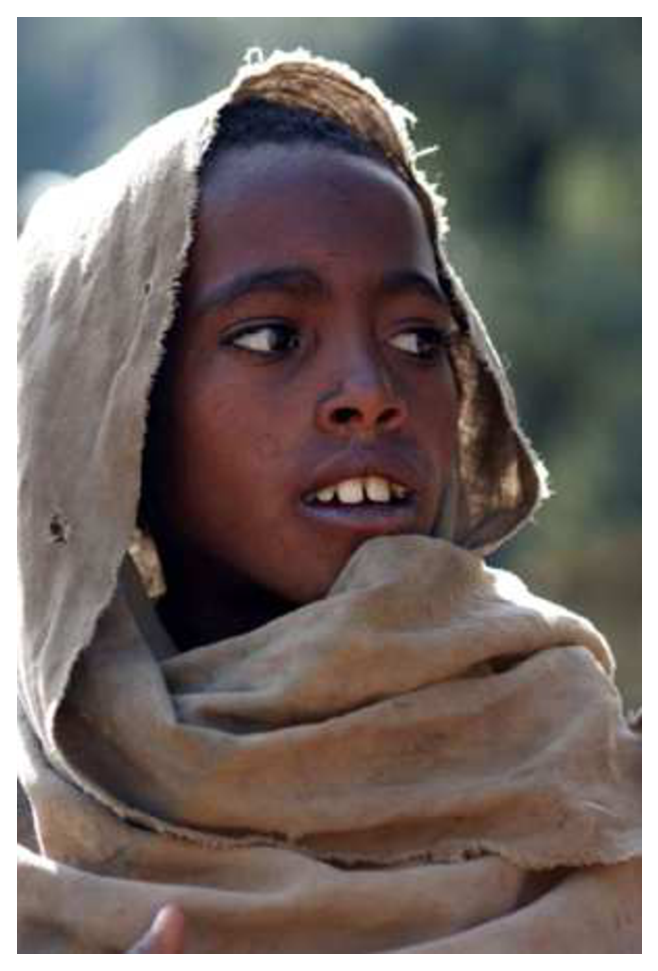
\includegraphics{etiopan.eps}\reflectbox{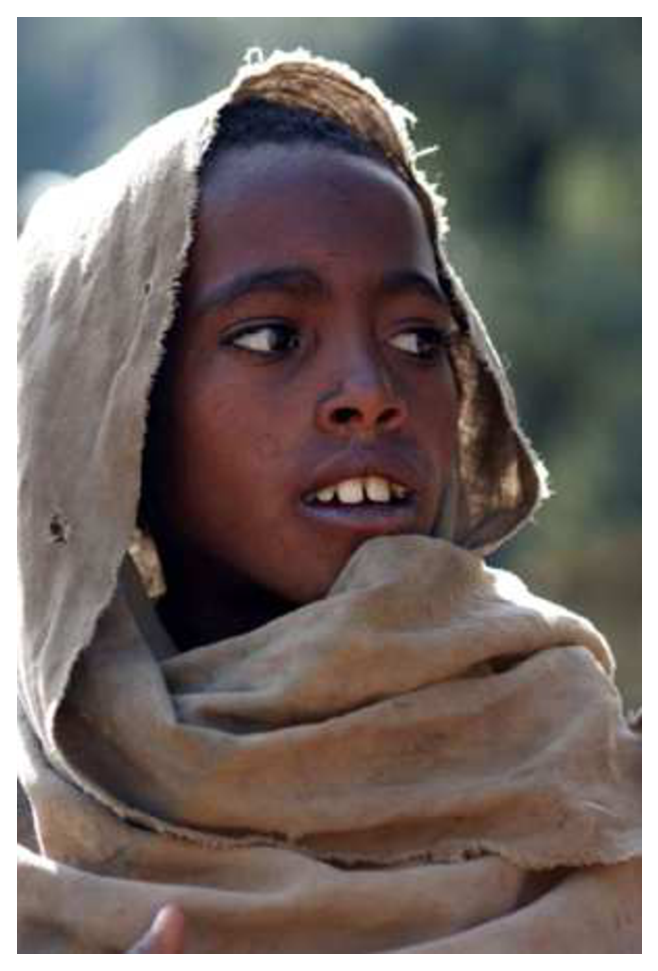
\includegraphics{etiopan.eps}}}
\caption{Malý Etiopánek a jeho bratříček}
\label{img:etiopanek}
\end{figure}

Rozdíl mezi vektorovým\dots

\begin{figure}
\scalebox{0.33}{
\includegraphics{oniisan.eps}}
\caption{Vektorový obrázek}
\label{img:oniisanvector}
\end{figure}

\dots a bitmapovým obrázkem

\begin{figure}
\scalebox{0.33}{
\includegraphics{oniisan2.eps}}
\caption{Bitmapový obrázek}
\label{img:oniisanbitmap}
\end{figure}

se projeví například při zvětšení.\par
Odkazy (nejen ty) na obrázky ODKAZ1, ODKAZ2, ODKAZ3, na tabulky ODKAZ1 a ODKAZ2 a také na algoritmus ODKAZ1 jsou udělány pomocí křížových odkazů. Pak je ovšem potřeba zdrojový soubor přeložit dvakrát.\par
Vektorové obrázky lze vytvořit i přímo v \LaTeX u, například pomocí prostředí \verb|picture|.
\end{document}